% Dokumentum beállítása
\documentclass[10pt]{beamer}
\usepackage{t1enc}
\usepackage[magyar]{babel}
\frenchspacing

% Téma beállítása
\usetheme{JuanLesPins} % Téma
\usecolortheme{Crane} % Téma színe
\usefonttheme{professionalfonts} % Betűtipus beállítása
\setbeamertemplate{navigation symbols}{} % Navigációs szimbólumok eltüntetése

% Outer/Inner theme beállítások
\useoutertheme{infolines} % Külső téma
\useinnertheme{rectangles} % Belső téma

% Szükséges csomagok
\usepackage{media9} % Videó csomag
\usepackage{graphicx} % Képek és Grafikák
\usepackage{xcolor} % Színek
\usepackage{hyperref} % Hyperhivatkozások
\usepackage{listings} % Kód blokkok kezelése és szép megjelenítése
\usepackage{tikz} % TikZ ábrák kezelése
\usepackage{pgf-pie} % Kördiagram TikZ-hez
\usepackage{multicol} % Több oszlopos elrendezés kezelése
\usepackage{wrapfig} % A szöveg a körbefuttatása
\usepackage{array}
\usepackage{longtable} % Többsoros táblázat

% Egyéni szín létrehozása
\definecolor{hyperpurple}{RGB}{89, 41, 134}

% "Dummy" szintaxis regisztrálása a listings csomagnak.
\lstdefinelanguage{Dummy}{ morekeywords={}, sensitive=true, comment=[l]{}, morestring=[b]", morestring=[b]' }

\lstset { % A listings csomag beállításai
    showstringspaces=false
}

% Hyperlink "hyper purple" szín + aláhúzás parancs létrehozása
\newcommand{\hyperstyle}[1]{{\color{hyperpurple}\underline{#1}}}

% Fő dokumentum kezdete
\begin{document}
	\begin{frame}
		\title{A Programozás mint hobbi, mint tanulmány}
		\author{Cser Máté | Neptun kód: HR8LLC}
		\date{\today}

		\titlepage % Cím dia
	\end{frame}

	% Tartalom jegyzék
	\begin{frame}
		\frametitle{Tartalomjegyzék}
		\setcounter{tocdepth}{1}
		\tableofcontents[pausesections]
	\end{frame}

	% Előzetes videó
	\begin{frame}
		\frametitle{Bevezető videó}

		% Videó beágyazása
		\includemedia[width=1\linewidth, height=0.45\linewidth,
		label=into-video.mp4 ]{}{VPlayer.swf} \pause
	\end{frame}

	% Dia (Bevezetés)
	\section{Bevezetés}
	\begin{frame}
		\frametitle{Programozás mint hobbi}

		\transdissolve \hspace{0.25cm} Szerintem a programozás nagyszerű hobbi, mivel
		fejleszti a Logikus gondolkodást, illetve segít a kreativitásunk
		megalkotásában. \pause

		\vspace{0.5cm}
		\hspace{0.25cm} Már régebb óta foglalkozok kisebb programok, applikációk és scriptek
		írásával, mivel már kisebb korom óta érdekel a programozás. \pause

		Jelenleg a leggyakrabban használt programozási nyelveim:

		\transdissolve
		\begin{itemize}
			\item \hyperstyle{ \hyperlink{java}{Java} } \pause

			\item \hyperstyle{ \hyperlink{lua}{Lua} } \pause

			\item \hyperstyle{ \hyperlink{nodejs}{Node.js} } \pause

			\item \hyperstyle{ \hyperlink{php}{PHP} } \pause
		\end{itemize}
	\end{frame}

	\transboxin
	% Dia (Java)
	\section{A Java nyelv}
	\subsection{Bevezetés a Java nyelvbe}
	\begin{frame}
		\frametitle{A Java nyelv}
		\hypertarget{java}{}

		% Java logo
		\begin{wrapfigure}
			{l}{0.12\textwidth}
			
\includegraphics[height=0.2\textwidth]{java-logo.png} % Java Logo
		\end{wrapfigure}

		% Szöveg
		\hspace{0.25cm} A Java egy általános célú, objektumorientált programozási
		nyelv, amelyet a Sun Microsystems fejlesztett a ’90-es évek elejétől kezdve egészen
		2009-ig, amikor a céget felvásárolta az Oracle. \pause

		\vspace{0.5cm}
		\hspace{0.25cm} A Java alkalmazásokat jellemzően bájtkód formátumra
		alakítják, de közvetlenül natív (gépi) kód is készíthető Java forráskódból.
		A bájtkód futtatása a Java virtuális géppel történik (JVM), ami vagy interpretálja
		a bájtkódot, vagy natív gépi kódot készít belőle, és azt futtatja az adott operációs
		rendszeren. \pause

		% Info block
		\vspace{1cm}
		\begin{block}{Info}
			Létezik közvetlenül Java bájtkódot futtató hardver is, az úgynevezett Java
			processzor.
		\end{block}
	\end{frame}

	% Dia (Java kód)
	\subsection{Példa kód}
	\begin{frame}[fragile]
		\frametitle{Java nyelv "Helló világ" Példa}

		Az alábbi példa a System.out.println funkció segítségével, a konzolunkba ki írja,
		hogy "Hello, World!". \begin{lstlisting}[language=Java]
    public class HelloWorld {
        public static void main(String[] args) {
            System.out.println("Hello, World!");
        }
    }
  \end{lstlisting}
	\end{frame}

	% Dia (Java előnyök, hátrányok)
	\subsection{Java előnyei, hátrányai}
	\begin{frame}
		\frametitle{A Java nyelv előnyei és hátrányai}

		\begin{block}{Előnyei}
			Nagy teljesítmény és skálázhatóság. \\ Multithreading és párhuzamos
			feldolgozás.
		\end{block}
		\begin{alertblock}{Hátrányai}
			Magas memória használat. \\ Hosszú hibakódok, és lassú indítási idő (JVM
			inicializálás)
		\end{alertblock}
		\begin{exampleblock}{Példa a használatára}
			Android és Játék fejlesztés például: \hyperstyle{\href{https://www.minecraft.net/en-us}{Minecraft}}.
			\\ Nagyvállalati alkalmazások, például bank rendszerek.
		\end{exampleblock}
	\end{frame}

	\transboxin
	% Dia (Lua)
	\section{A Lua nyelv}
	\subsection{Bevezetés a Lua nyelvbe}
	\begin{frame}
		\frametitle{A Lua nyelv}
		\hypertarget{lua}{}

		% Lua logo
		\begin{wrapfigure}
			{r}{0.15\textwidth}
			
\includegraphics[height=0.15\textwidth]{lua-logo.png} % Lua Logo
		\end{wrapfigure}

		% Szöveg
		\hspace{0.25cm} A Lua\\(portugálul jelentése: Hold), egy nyílt forráskódú,
		beágyazható szkriptnyelv, amelyet 1993-ban fejlesztettek ki a brazíliai Katolikus
		Teológiai Egyetemen. \pause
		
		\vspace{0.5cm}
		A készítői fontosnak tartották az
		együttműködését a C nyelvű programokkal, programkönyvtárakkal.
		Platformfüggetlen, a programok futási idő előtt bájtkódra fordulnak. \pause

		% Info block
		\vspace{1cm}
		\begin{block}{Info}
			Bár önállóan is használható, de leginkább beágyazva találjuk meg más
			szoftverekben.
		\end{block}
	\end{frame}

	% Dia (Lua kód)
	\subsection{Példa kód}
	\begin{frame}[fragile]
		\frametitle{Lua nyelv "Helló világ" Példa}

		Az alábbi példa a Lua beépített print funkció segítségével, a konzolunkba ki
		írja, hogy "Hello, World!". \begin{lstlisting}[language=Dummy]
    print("Hello, World!")
  \end{lstlisting}
	\end{frame}

	% Dia (Lua előnyök, hátrányok)
	\subsection{Lua előnyei, hátrányai}
	\begin{frame}
		\frametitle{A Lua nyelv előnyei és hátrányai}

		\begin{block}{Előnyei}
			Könnyen tanulható és a szintaxisa egyszerű. \\ Könnyen beágyazható más
			alkalmazásokba.
		\end{block}
		\begin{alertblock}{Hátrányai}
			Nem annyira gyors mint a Java vagy a C++. \\ Korlátozottak a beépített
			funkciói
		\end{alertblock}
		\begin{exampleblock}{Példa a használatára}
			Játékon belüli szkriptelés/játéktartalom fejlesztés, például: \hyperstyle{\href{https://www.roblox.com}{Roblox}},
			\hyperstyle{\href{https://store.steampowered.com/app/4000/Garrys_Mod/}{Garry's Mod}}.
			\\ Kisebb alkalmazások, eszközök automatizálása, makrók szkriptelése.
		\end{exampleblock}
	\end{frame}

	\transboxin
	% Dia (Node.js)
	\section{A Node.js nyelv}
	\subsection{Bevezetés a Node.js nyelvbe}
	\begin{frame}
		\frametitle{A Node.js nyelv}
		\hypertarget{nodejs}{}

		% Java logo
		\begin{wrapfigure}
			{l}{0.2\textwidth}
			
\includegraphics[height=0.12\textwidth]{nodejs-logo.png} % NodeJS Logo
		\end{wrapfigure}

		% Szöveg
		\hspace{0.25cm} A Node.js egy szoftverrendszer, melyet skálázható internetes
		alkalmazások mégpedig webszerverek készítésére hoztak létre.\pause

		\vspace{0.5cm}
		\hspace{0.25cm} A Node.js-t Ryan Dahl hozta létre 2009 januárjában, a
		növekedését a pedig Poyent Dahl munkaadója támogatja.\pause

		\vspace{0.5cm}
		\hspace{0.25cm} Dahl célja az volt, hogy lehessen weboldalakat push
		technológiával létrehozni. Számos egyéb más programnyelvekben való próbálkozás
		után a JavaScriptet választotta a meglévő I/O API hiánya miatt. \pause

		% Info block
		\vspace{1cm}
		\begin{block}{Info}
			Hasonlókat írtak már más programnyelvekre is, például a Twistedet Pythonra,
			Perl Object Enviromentet Pearlhez, vagy a libeventet C nyelvhez.
		\end{block}
	\end{frame}

	% Dia (Node.js kód)
	\subsection{Példa kód}
	\begin{frame}[fragile]
		\frametitle{Node.js nyelv "Helló világ" példa}

		Az alábbi példa ki-írja a node.js konzolba, a console.log funkció segítségével,
		hogy "Hello World!".
		\begin{lstlisting}[language=Dummy]
    console.log("Hello, World!")
  \end{lstlisting}
	\end{frame}

	% Dia (Node.js előnyök, hátrányok)
	\subsection{Node.js előnyei, hátrányai}
	\begin{frame}
		\frametitle{A Node.js nyelv előnyei és hátrányai}

		\begin{block}{Előnyei}
			Nagy közösség és rengeteg csomag. \\ Aszinkron feldolgozás (nem blokkoló I/O).
		\end{block}
		\begin{alertblock}{Hátrányai}
			Egy szálon fut, nem ideális CPU-intenzív feladatokra. \\ Nem mindegyik közösség
			által készített csomag van karbantartva vagy dokumentálva
		\end{alertblock}
		\begin{exampleblock}{Példa a használatára}
			Ideális webalkalmazáso és real-time alkalmazások készítéséhez mint például:
			Chat vagy Multiplayer Játékok, és a full-stack fejlesztéshez.
		\end{exampleblock}
	\end{frame}

	% Dia (Node.js leghíresebb NPM csomagok)
	\subsection{Leghíresebb Node.js csomagok}
	\begin{frame}
		\frametitle{Leghíresebb NPM csomagok}

		\begin{multicols}{3}
			\begin{itemize}
				\transglitter

				\item 1. Express

				\item 2. Async

				\item 3. Lodash

				\item 4. Cloudinary \pause \transglitter

				\item 5. Axios

				\item 6. Karma

				\item 7. Molecular

				\item 8. Grunt \pause \transglitter

				\item 9. PM2

				\item 10. Mocha

				\item 11. Moment

				\item 12. Babel
			\end{itemize}
		\end{multicols}
	\end{frame}

	\transboxin
	% Dia (PHP)
	\section{A PHP nyelv}
	\subsection{Bevezetés a PHP nyelvbe}
	\begin{frame}
		\frametitle{A PHP nyelv}
		\hypertarget{php}{}

		% Java logo
		\begin{wrapfigure}
			{r}{0.22\textwidth}
			
\includegraphics[height=0.15\textwidth]{php-logo.png} % Java Logo
		\end{wrapfigure}

		% Szöveg
		\hspace{0.25cm} A PHP egy általános szerveroldali szkriptnyelv dinamikus weblapok
		készítésére. \pause

		\vspace{0.5cm}
		\hspace{0.25cm} Az első szkriptnyelvek egyike, amely külső fájl használata
		helyett HTML oldalba ágyazható. \pause

		\vspace{0.5cm}
		\hspace{0.25cm} Rasmus Lerdorf 1995-ben indította útjára, ma a The PHP Group
		tartja fenn és fejleszti a projektet, A PHP születésekor csupán egy
		makrókészlet volt személyen honlapok karbantartására, innen jön az eredeti neve:
		"Peronal Home Page Tools", később a rövidítés jelentése "Hypertext
		Preprocessor" lett. \pause

		% Info block
		\vspace{1cm}
		\begin{block}{Info}
			A HTML oldalba ágyazott kódot a webszerver PHP feldolgozómotorja értelmezi,
			ezzel dinamikus oldalakat hozva létre..
		\end{block}
	\end{frame}

	% Dia (PHP kód)
	\subsection{Példa kód}
	\begin{frame}[fragile]
		\frametitle{Node.js nyelv "Helló világ" példa}

		Az alábbi példa egy PHP által készített dinamikus weboldal, amely megnyitáskor
		kiírja, hogy "Hello World!".
		\begin{lstlisting}[language=PHP]
  <?php echo("Hello, World!);?>
\end{lstlisting}
	\end{frame}

	% Dia (PHP előnyök, hátrányok)
	\subsection{PHP előnyei, hátrányai}
	\begin{frame}
		\frametitle{A PHP nyelv előnyei és hátrányai}

		\begin{block}{Előnyei}
			Sokféle eszköz és framework elérhető hozzá, mint a Laravel vagy a Symfony
			\\ Erőteljes és buzgó közössége van amely folyamatosan aktív, így rengeteg
			könyvtár, framework és támogatottság áll rendelkezésre.
		\end{block}
		\begin{alertblock}{Hátrányai}
			Biztonsági problémák, rosszul megírt kód, vagy régebbi verzió esetében \\ A
			PHP gyors, de nem versenyképes más nyelvekkel min a Python vagy a Node.js
		\end{alertblock}
		\begin{exampleblock}{Példa a használatára}
			A PHP ideális szerver-oldalú adatok kezelésére, mint például űrlapok
			feldolgozására, fájlkezelés és adatbázis műveletekhez, illetve
			tartalomkezelő rendszerekhez.
		\end{exampleblock}
	\end{frame}

	% Dia (PHP legismertebb csomagjai)
	\subsection{PHP legismertebb csomagjai és leírása}
	\begin{frame}
		\frametitle{A PHP legismertebb csomagjai, használata és leírása}

		\begin{tabular}{|l|l|>{\raggedright\arraybackslash}m{6.4cm}|}
			\hline
			Csomag neve & Használati helye & Leírása                                                                                                     \\
			\hline
			Composer    & Csomagkezelés    & A PHP legnépszerűbb csomagkezelő eszköze, amely lehetővé teszi a könyvtárak és függőségek könnyű kezelését. \\
			\hline
			Laravel     & Keretrendszer    & Egy modern PHP framework amely MVC (Model-View-Controller) alapú fejlesztést tesz lehetőbe.                 \\
			\hline
			Symfony     & Keretrendszer    & Nagy teljesítményű, robusztus PHP framework, amelyet az vállalati szintű alkalmazásokhoz fejlesztettek.     \\
			\hline
			Guzzle      & HTTP Kliens      & Egy erőteljes HTTP kliens könyvtár, amely segíti a HTTP requestek kezelését és API-k használatát.           \\
			\hline
		\end{tabular}
	\end{frame}

	\section{Nyelvek elterjedtsége}
	\begin{frame}
		\frametitle{Az egyes nyelvek elterjedtsége}

		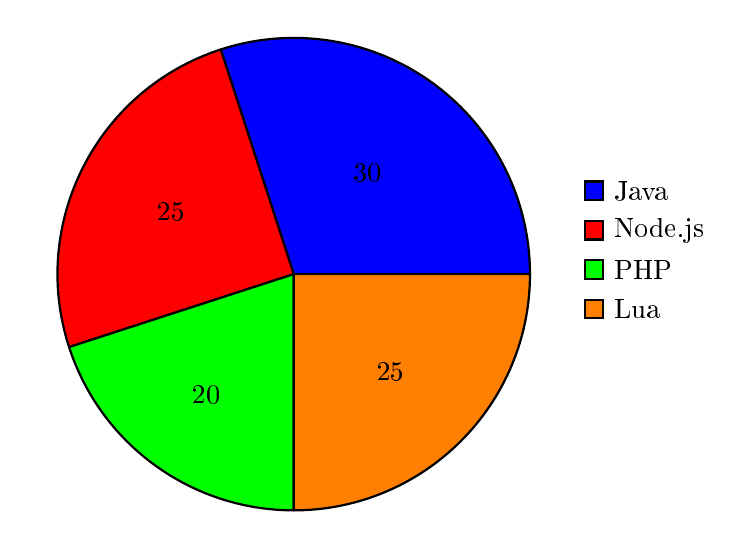
\begin{tikzpicture}
			\pie[sum=auto, text=legend, radius=3, color={blue, red, green, orange}]{ 30/Java, 25/Node.js, 20/PHP, 25/Lua }
		\end{tikzpicture}
	\end{frame}

	% Összefoglaló Dia
	\transboxin
	\section{Összefoglaló}
	\subsection{1/2 Összefoglaló}
	\begin{frame}
		\frametitle{A nyelvek rövid összefoglaló 1/2}

		\begin{itemize}
			\item Java
				\begin{itemize}
					\item Előnyei
						\begin{itemize}
							\item Platform független a JVM segítsége miatt.

							\item Erős a típus ellenőrzése és robosztus a kódolása.
						\end{itemize}

					\item Hátrányai
						\begin{itemize}
							\item Bonyolult szintaxis és ezáltal nehezen tanulható.

							\item Lassú az indítása és magas a memória használata az alkalmazásoknak.
						\end{itemize}
				\end{itemize}

			\item Node.js
				\begin{itemize}
					\item Előnyei
						\begin{itemize}
							\item Nagy a sebessége és jól skálázható.

							\item Aszinkron és nem blokkoló az I/O feldolgozása.
						\end{itemize}

					\item Hátrányai
						\begin{itemize}
							\item Egy szálú, így nem használható nagy CPU-t igényű feladatokra.

							\item Nehéz a hibakeresés, és gyorsan callback hell lesz a sok
								callbackek használat miatt az aszinkronsága miatt.
						\end{itemize}
				\end{itemize}
		\end{itemize}
	\end{frame}
	\transdissolve
	\subsection{2/2 összefoglaló}
	\begin{frame}
		\frametitle{A nyelvek rövid összefoglalója 2/2}

		\begin{itemize}
			\item PHP
				\begin{itemize}
					\item Előnyei
						\begin{itemize}
							\item Webfejlesztésre optimalizált,könnyen kezelhető adatbázis kezelési
								funkciókkal.

							\item Széles körű a közössége, így sok csomag és eszköz elérhető.
						\end{itemize}

					\item Hátrányai
						\begin{itemize}
							\item Alacsony és lassú teljesítmény komplex alkalmazásoknál.

							\item Biztonsági problémák keletkezhetnek, ha a verzió régi, vagy ha
								nem megfelelően használják.
						\end{itemize}
				\end{itemize}

			\item Lua
				\begin{itemize}
					\item Előnyei
						\begin{itemize}
							\item Kicsi és gyors, kevés az erőforrás igénye.

							\item Egyszerű a szintaxisa és könnyen tanulható.
						\end{itemize}

					\item Hátrányai
						\begin{itemize}
							\item Kevés a beépített könyvtár és a funkcionalitása.

							\item Nem ideális és használható nagy vagy komplex alkalmazásokhoz
						\end{itemize}
				\end{itemize}
		\end{itemize}
	\end{frame}
	
	\transdissolve
	\section{Algoritmusok komplexitása}
	% Komplexitás
	\begin{frame}
		\frametitle{Algoritmusok komplexitása}
		
		Egyes algoritmusok komplexitása gyakran:\\
		\[O(n)\], \[O(n^2)\], vagy akár \[O(\log(n))\], de akár bonyolultabb függvényekkel is lehet a háttérben futó műveletek alapján.
	\end{frame}

	% Forrás jegyzék
	\begin{frame}
		\frametitle{Forrásjegyzék}

		\begin{thebibliography}{9}
			\bibitem{intro} Pixabay.com, \emph{Bevezető videó},
				\url{https://pixabay.com/videos/countdown-reveal-timer-counter-93824}		
		
			\bibitem{lua} Lua.org, \emph{Lua weboldala},
				\url{https://www.lua.org}

			\bibitem{java} Oracle, \emph{Java weboldala},
				\url{https://www.oracle.com/java}

			\bibitem{nodejs} Node.js Foundation, \emph{Node.js weboldala},
				\url{https://nodejs.org}
				
			\bibitem{php} The PHP Group, \emph{PHP weboldala},
				\url{https://php.net}
				
			\bibitem{other} Egyéb források,
				\url{https://hu.wikipedia.org/wiki/}
		\end{thebibliography}
	\end{frame}
	
	% Vége
	\begin{frame}
		\begin{center}
			\textbf{\huge{VÉGE}} \\
			\textsc{ \large{ Köszönöm a figyelmet! } }
		\end{center}
	\end{frame}
\end{document}